%\documentclass[dvipdfmx]{beamer}      % platex の場合
\documentclass[handout]{beamer}        % lualatex の場合
\usepackage{mySld}
\usepackage{multicol}

\begin{document}
\title{基礎コンピュータ工学\\第5章 機械語プログラミング\\(パート8)}
\date{}

\begin{frame}
  \titlepage
  \centerline{\url{https://github.com/tctsigemura/TecTextBook}}
  \vfill
  \centerline{本スライドの入手:
    \raisebox{-7mm}{
\includegraphics[scale=0.3]{../Img/QRs5_8.png}}}
\end{frame}

%==============================================================================
%\begin{frame}
%  \frametitle
%  \tableofcontents
%\end{frame}

\section{シフト(桁ずらし)命令}
%==============================================================================
\begin{frame}
  \frametitle{シフト(桁ずらし)命令}
  \begin{itemize}
  \item データの2進数を左右に桁移動する命令のこと.
  \item TeCは4種類(実質は3種類)の命令を持っている.
  \item \emph{左シフト(論理・算術)}\\
    \vspace{-0.3cm}\centerline{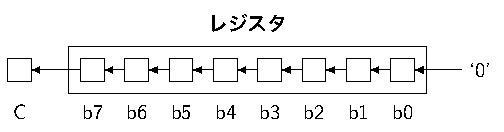
\includegraphics[scale=0.7]{../Tikz/shft1.pdf}}
  \item \emph{右シフト(論理)}\\
    \centerline{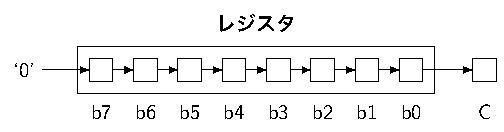
\includegraphics[scale=0.7]{../Tikz/shft3.pdf}}
  \item \emph{右シフト(算術)}\\
    \centerline{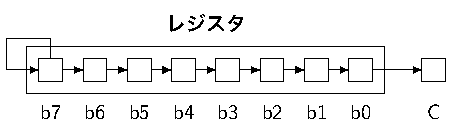
\includegraphics[scale=0.7]{../Tikz/shft2.pdf}}
  \end{itemize}
  \vfill
\end{frame}

%==============================================================================
\begin{frame}
  \frametitle{SHLA(Shift Left Arithmetic)命令}
  左算術(算術=Arithmetic)シフト命令.\\
  レジスタの値を左に\emph{1ビット}ずらす.(シフトする)\\
  \vfill
  \centerline{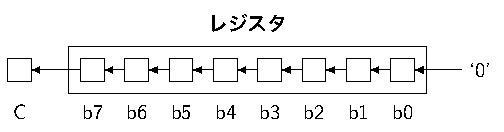
\includegraphics[scale=0.7]{../Tikz/shft1.pdf}}
  \vfill
  \begin{description}
  \item[Cフラグ] 上の図のように変化する.
  \item[Sフラグ] 結果が負なら1,それ以外は0になる.
  \item[Zフラグ] 結果がゼロなら1,それ以外は0になる.
    \vfill
  \item[フローチャート:] Javaのシフト演算子を流用する.\\
    \centerline{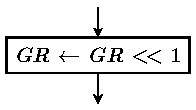
\includegraphics[scale=0.7]{../Tikz/shla.pdf}}
  \end{description}
  \vfill
\end{frame}

%==============================================================================
\begin{frame}
  \begin{description}
  \item[ニーモニック:] \texttt{SHLA GR}
    \vfill
  \item[命令フォーマット:] 1バイトの長さを持つ.\\
    \oneByte{$1001_2$}{\GR~$00_2$}
  \end{description}
  \vfill
  \vfill
  \emph{例:}SHLA命令を実行して確かめる.(イルミネーション?)\\
  (次のプログラムをG0を表示したままSTEP実行する.)
  \vfill
  \centerline{\ttfamily %\footnotesize
    \begin{tabular}{|l|l|l|l|l|}
      00 & 10 05 &      & LD   & G0, N    \\
      02 & 90    & LOOP & SHLA & G0       \\
      03 & A0 02 &      & JMP  & LOOP     \\
      05 & 01    & N    & DC   & 1        \\
    \end{tabular}}
  \vfill
  \emph{注:}左シフトは×2を計算している.\\
  \vfill
\end{frame}

%==============================================================================
\begin{frame}
  \frametitle{SHLL(Shift Left Logical)命令}
  左論理(論理=Logical)シフト命令.\\
  レジスタの値を左に\emph{1ビット}ずらす.(シフトする)\\
  (SHLL命令とSHLA命令の動作は全く同じ.)
  \vfill
  \begin{description}
  \item[フラグ] SHLAと同じ
    \vfill
  \item[フローチャート:] SHLAと同じ
    \vfill
  \item[ニーモニック:] \texttt{SHLL GR}
    \vfill
  \item[命令フォーマット:] 1バイトの長さを持つ.\\
    \oneByte{$1001_2$}{\GR~$01_2$}
  \end{description}
  \vfill
\end{frame}

%==============================================================================
\begin{frame}
  \frametitle{左シフトを用いた×2計算}
  \begin{minipage}{0.48\columnwidth}
    \begin{center}
      {\ttfamily%\footnotesize
        \begin{tabular}{r r}
          \multicolumn{2}{c}{符号なし数の×2} \\
          0000 0001 & (1) \\
          0000 0010 & (2) \\
          0000 0100 & (4) \\
          0000 1000 & (8) \\
          0001 0000 & (16) \\
          0010 0000 & (32) \\
          0100 0000 & (64) \\
          1000 0000 & (128) \\
          0000 0000 & (ERR) \\
        \end{tabular}
      }\\
      \vspace{0.5cm}
      SHLL命令はこちら用
    \end{center}
  \end{minipage}
  \begin{minipage}{0.48\columnwidth}
    \begin{center}
      {\ttfamily%\footnotesize
        \begin{tabular}{r r}
          \multicolumn{2}{c}{符号付き数の×2} \\
          1111 1111 & (-1) \\
          1111 1110 & (-2) \\
          1111 1100 & (-4) \\
          1111 1000 & (-8) \\
          1111 0000 & (-16) \\
          1110 0000 & (-32) \\
          1100 0000 & (-64) \\
          1000 0000 & (-128) \\
          0000 0000 & (ERR) \\
        \end{tabular}
      }\\
      \vspace{0.5cm}
      SHLA命令はこちら用
    \end{center}
  \end{minipage}
  \vfill
\end{frame}

%==============================================================================
\begin{frame}
  \frametitle{SHRA(Shift Right Arithmetic)命令}
  右算術(算術=Arithmetic)シフト命令.\\
  レジスタの値を右に\emph{1ビット}ずらす.(シフトする)
  \vfill
  \centerline{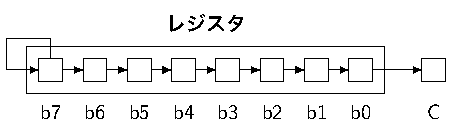
\includegraphics[scale=0.7]{../Tikz/shft2.pdf}}
  \vfill
  \begin{description}
  \item[フラグ] SHLAと同じ
    \vfill
  \item[フローチャート:] Javaのシフト演算子を流用する.\\
    \centerline{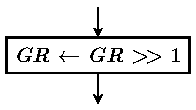
\includegraphics[scale=0.7]{../Tikz/shra.pdf}}
    \vfill
  \item[命令フォーマット:] 1バイトの長さを持つ.\\
    \oneByte{$1001_2$}{\GR~$10_2$}
  \item[注:] SHRAは符号付き数の÷2を計算している.\\
  \end{description}
  \vfill
\end{frame}

%==============================================================================
\begin{frame}
  \frametitle{SHRL(Shift Right Logical)命令}
  右論理(論理=Logical)シフト命令.\\
  レジスタの値を右に\emph{1ビット}ずらす.(シフトする)
  \vfill
  \centerline{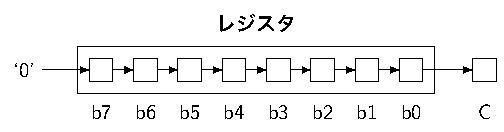
\includegraphics[scale=0.7]{../Tikz/shft3.pdf}}
  \vfill
  \begin{description}
  \item[フラグ] SHLAと同じ
    \vfill
  \item[フローチャート:] Javaのシフト演算子を流用する.\\
    \centerline{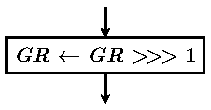
\includegraphics[scale=0.7]{../Tikz/shrl.pdf}}
    \vfill
  \item[命令フォーマット:] 1バイトの長さを持つ.\\
    \oneByte{$1001_2$}{\GR~$11_2$}
  \item[注:] SHRLは符号なし数の÷2を計算している.\\
  \end{description}
  \vfill
\end{frame}

%==============================================================================
\begin{frame}
  \frametitle{右シフトを用いた÷2計算(1)}
  \begin{minipage}{0.48\columnwidth}
    \begin{center}
      {\ttfamily%\footnotesize
        \begin{tabular}{r r}
          \multicolumn{2}{c}{符号なし数の÷2} \\
          1100 0000 & (192) \\ % 128+64=192
          0110 0000 & (96)  \\ % 64+32=96
          0011 0000 & (48)  \\ % 32+16=48
          0001 1000 & (24)  \\ % 16+8=24
          0000 1100 & (12)  \\ % 8+4=12
          0000 0110 & (6)   \\
          0000 0011 & (3)   \\
          0000 0001 & (1)   \\
          0000 0000 & (0)   \\
        \end{tabular}
      }\\
      \vspace{0.5cm}
      SHRL命令を使用する
    \end{center}
  \end{minipage}
  \begin{minipage}{0.48\columnwidth}
    \begin{center}
      {\ttfamily%\footnotesize
        \begin{tabular}{r r}
          \multicolumn{2}{c}{符号付き数の÷2} \\
          1100 0000 & (-64) \\
          1110 0000 & (-32) \\
          1111 0000 & (-16) \\
          1111 1000 & (-8)  \\
          1111 1100 & (-4)  \\
          1111 1110 & (-2)  \\
          1111 1111 & (-1) \\
          1111 1111 & (-1) \\
          1111 1111 & (-1) \\
        \end{tabular}
      }\\
      \vspace{0.5cm}
      SHRA命令を使用する
    \end{center}
  \end{minipage}
  \vfill
\end{frame}

%==============================================================================
\begin{frame}
  \frametitle{右シフトを用いた÷2計算(2)}
  \begin{minipage}{0.48\columnwidth}
    \begin{center}
      {\ttfamily%\footnotesize
        \begin{tabular}{r r}
          \multicolumn{2}{c}{符号付き正数の÷2} \\
          0100 0000 & (64) \\
          0010 0000 & (32) \\
          0001 0000 & (16) \\
          0000 1000 & (8)  \\
          0000 0100 & (4)  \\
          0000 0010 & (2)  \\
          0000 0001 & (1)  \\
          0000 0000 & (0)  \\
          0000 0000 & (0)  \\
        \end{tabular}
      }\\
      \vspace{0.5cm}
      SHRA命令使用
    \end{center}
  \end{minipage}
  \begin{minipage}{0.48\columnwidth}
    \begin{center}
      {\ttfamily%\footnotesize
        \begin{tabular}{r r}
          \multicolumn{2}{c}{符号付き負数の÷2} \\
          1100 0000 & (-64) \\
          1110 0000 & (-32) \\
          1111 0000 & (-16) \\
          1111 1000 & (-8)  \\
          1111 1100 & (-4)  \\
          1111 1110 & (-2)  \\
          1111 1111 & (-1)  \\
          1111 1111 & (-1)  \\
          1111 1111 & (-1)  \\
        \end{tabular}
      }\\
      \vspace{0.5cm}
      SHRA命令使用
    \end{center}
  \end{minipage}
  \vfill
\end{frame}

%==============================================================================
\begin{frame}
  \frametitle{まとめ}
  \emph{学んだこと}
  \begin{itemize}
  \item TeCのシフト命令は\emph{1ビット}シフトする.
  \item TeCは4種類(実質は3種類)のシフト命令を持っている.
  \item シフト命令はイルミネーション(?)に使用できる.
  \item \emph{左シフト(論理・算術)}は,\\
    符号付き・なし兼用の×2計算に使用できる.
  \item \emph{右シフト(論理)}は,
    符号なし数の÷2計算に使用できる.
  \item \emph{右シフト(算術)}は,
    符号付き数の÷2計算に使用できる.
  \end{itemize}
  \vfill
  \emph{演習}
  \begin{itemize}
  \item ビットの右回転(例題5−5を参考に)
  \item シフト命令を使用した「×7の計算」(例題5−6を参考に)
  \item シフト命令を使用した「÷4の計算」
  \item シフト命令を使用した「×1.5の計算」
  \end{itemize}
  \vfill
\end{frame}

\end{document}
